\chapter{Literature Review}
% -_____________________________________________________________________________

This section introduces the foundations of blockchain systems and Ethereum to the reader before acquainting them with the current state of research in the field.

The terms '\textbf{power}' and '\textbf{energy}' refer to \textbf{electrical energy} through this study. 

% -_____________________________________________________________________________

\section{Blockchain Basics}

Blockchain has been recognised as a transformative innovation in many industries beyond cryptocurrencies, such as  healthcare, Internet of Things (IoT), logistics and especially finance. It was first introduced in 2008 by Nakamoto \cite{NakamotoBitcoin:System}. Compared to traditional centralised systems, blockchain offers several distinct advantages, including immutability, heightened security, fault tolerance, transparency and it gives users a greater level of control, all through decentralisation.

\subsection{How it works}

A blockchain is similar to a linked list in that it consists of a series of blocks containing transaction information. Each block is linked to the one before it using deterministic cryptographic hashes, forming an immutable chain of blocks that hold hashed information which cannot be altered. This chain of blocks is also known as the public \textbf{ledger}, depicted in \fref{Figure:BasicBlockchain}. Altering any of the blocks in this ledger will invalidate the hashes of all the blocks after it, making blockchain technology resistant to data modification. Computers choosing to participate in a blockchain network are called \textbf{nodes}, each of which hold a copy of the public ledger. This ledger is updated as new transaction information is received by the node, which is also responsible for propagating it to the rest of the network.

\begin{figure}[h]
    \centering
    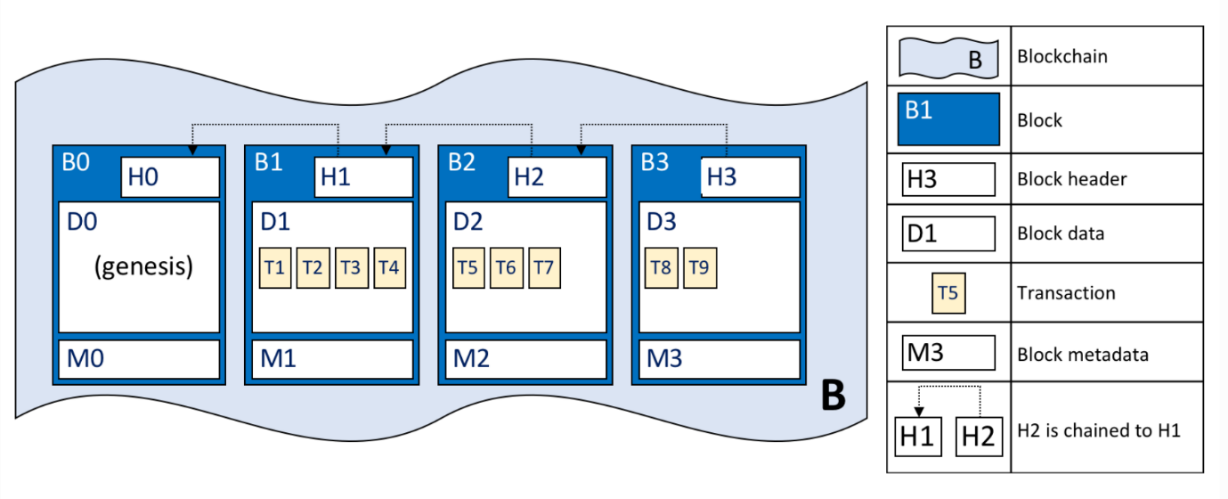
\includegraphics[width=13cm,center]{Figures/BlockchainStructure.png}
    \caption{The data structure underlying blockchain. The first block is called the Genesis Block. Source: \cite{ADocumentation}.}
    \label{Figure:BasicBlockchain}
\end{figure}

The public ledger is a decentralised data structure that serves as the single source of truth to all nodes on the network creating trust between anonymous actors. This removes the need for an intermediary, like a bank, to mediate a transaction between 2 parties. External authorities are not required to validate the authenticity and integrity of data either.



% -_____________________________________________________________________________

\subsection{Consensus Protocols}

The consensus protocol determines how nodes validate and agree on any new transactions being permanently added to the public ledger, and it varies between different blockchains. It makes sure that all nodes in a network have a consistent view of the ledger. This mechanism plays a crucial role in safeguarding against a variety of attacks that malicious nodes could attempt.
% -_____________________________________________________________________________

\subsubsection{Proof-Of-Work}

PoW (Proof-Of-Work) is a type of consensus algorithm that couples voting weight with computing 
power. It relies on the network's computational resources to defend against the Sybil Attack \cite{Sedlmeir2020TheMyth}.

In PoW, nodes that actively chose to participate in the consensus-forming process are called \textbf{'miners'}. These miners compete 
to solve a computationally challenging mathematical puzzle in order to verify a group of transactions included in a block. 
% CAN BE CUT**
% In a brute-force manner, miners try to guess the right 'nonce' (number only used once) that when it is combined with the rest of the block header information and hashed, the hash has to have a certain number of leading zeros at the beginning. 
% ---
It is like trying to guess the number of a winning lottery ticket. It's challenging to produce (in terms of time and compute power) but easy to verify for other nodes \cite{Centieiro2021BitcoinCoding}. Once a node guesses the correct 'nonce', it proposes it to the rest of the network for validation. When most other miners have agreed on its legitimacy, the new block is permanently added to the blockchain ledger, and the block proposer is rewarded with mining fees and tips associated with those transactions.

% -_____________________________________________________________________________

\subsubsection{Proof-Of-Stake}

PoS (Proof-Of-Stake) is a newer consensus protocol that relies on economic power rather than computational power to secure the blockchain. In PoW, nodes choosing to participate in the consensus-forming process are called \textbf{'validators'}, which put up a set amount of their cryptocurrency at stake (as collateral). In exchange, they increase their chance of being randomly selected as the block proposer for the next round of transactions and consequently earn the block rewards that come with it \cite{King2012PPCoin:Proof-of-Stake}. In some implementations of PoS, the more a validator puts at stake, the higher their chance of being picked as the block proposer. Suppose a validator submits a fraudulent transaction or tampers with any transaction information. In that case, they risk losing their staked cryptocurrency and any block rewards they may have received, as other observing nodes always verify each new block \cite{Napoletano2022WhatAdvisor}. 

Compared to PoW, PoS is a much less energy-intensive mechanism by design.

% -_____________________________________________________________________________

% -_____________________________________________________________________________

\section{Introduction to Ethereum}

% Ethereum is an open-source blockchain platform that has grown to become the world's second largest blockchain (after Bitcoin) by market capitalisation. It was introduced in 2015 by Vitalik Buterin as a platform with capabilities beyond just cryptocurrency \cite{ButerinEthereum:Platform.}. It features smart contracts, which are self-executing programs that automatically activate when the specified criteria are met. The Ethereum blockchain forms the backbone for a variety of applications, including Decentralised Applications (DApps), thanks to the functionality of smart contracts.

Nodes that communicate following the 'ETH' protocol make up the Ethereum network, also called the Ethereum 'mainnet'. These nodes all contribute to maintaining and securing a globally agreed state of the Ethereum Virtual Machine (EVM). This was also described as 'one computer for the entire planet" by Ethereum co-founder Gavin Wood in 2016 \cite{Ethereum:Industries}. 

The security of this network comes from a majority of nodes agreeing on a new change to the current state of the EVM. In other words, agreeing on the next block to be permanently added to the blockchain ledger. Such consensus-forming nodes are paid in Ethereum's native cryptocurrency, \textbf{Ether (ETH)}, for running validator software that helps validate new blocks received over the peer-to-peer network.

% Ethereum is a public, permissionless network, which means that anyone can access and participate in its operations. 
% % ---
% The interaction between a client and the Ethereum blockchain is enabled by the JSON RPC(Remote Procedure Call) API. 
% % --
% When a user wants to complete a transaction with another user on the network, they:
% \begin{enumerate}
%     \item Need to specify the transaction amount
%     \item Secure the transaction with their own private key
%     \item Specify the tip they are willing to pay on top of the base transaction fees (defined in 'gas' units) to a validator to validate and include their transaction in an upcoming block
% \end{enumerate}

% The ETH Execution client verifies the transaction request by checking things like whether the user has enough ETH to complete the transaction and if they have used the correct private key etc. \cite{EthereumEthereum.org}. 
% This transaction request is then broadcasted to every other validator node over the execution layer 'gossip network'. Every validator adds this transaction to their local \textbf{'mempool'}. This is a collection of unverified transactions that are waiting to be processed and added to a new block.

During the pre-merge PoW era of Ethereum, \textbf{miners} used to compete 
% to solve a mathematical problem using their computational power, and the winner was rewarded with Ether and 
to earn the right to add a block to the blockchain 
% As more miners joined the network, the difficulty of the problem proportionally increased
, resulting in a computationally expensive and energy-intensive process.
% -_____________________________________________________________________________

% ________________________________________________________________________________-

% -_____________________________________________________________________________
\section{Post-Merge PoS Ethereum}

"The Merge", also known as the Paris Upgrade, took place on 15$\mathrm{^{th}}$ September 2022. The Ethereum Blockchain switched from the older Proof of Work (PoW) consensus protocol to Proof-of-Stake (PoS). The name "The Merge" derives from the fact that the Beacon Chain, a test network for Ethereum 2.0, was merged with the original Ethereum network. Both networks now operate simultaneously in layers. The old Ethereum chain is now referred to as the 'execution' layer (EL), now secured by the PoS 'consensus' layer (CL), formerly known as the Beacon Chain \cite{EthereumEthereum.org}. 

The merge of the original chain with the Beacon Chain made miners redundant. The Ethereum blockchain is now secured by \textbf{Validator Nodes}. 

\subsection{Types of Nodes}

The 4 main types of nodes include Full, Validator, Archive and Light Nodes. Archive nodes are designed to maintain an exact and complete copy of the entire ledger, dating back to the Genesis block. Light Nodes, on the other hand, offer a lightweight solution for users to interact with the Ethereum network, allowing for wider participation. The two remaining node types are discussed in detail below.

\subsubsection{Full Nodes}
There is a popular mantra in blockchain, "Don't trust, verify" \cite{EthereumEthereum.org}. Following this altruistic mantra, users running a Full Node can interact with the Ethereum network in a trustless and self-sufficient manner. Everything is checked and verified by your own node, helping to secure the network while removing the need to trust information received from other nodes. 

Full Nodes need to run both execution and consensus layer client software and must also be synchronised with the latest version of the public ledger in order to interact with the blockchain. 

To complete a transaction with another user on the network, users need to specify the amount in ETH, secure it with their private key, and set a tip for validators to incentivise them to include the transaction in an upcoming block.

The Ethereum EL client locally verifies the transaction request, ensuring the user has sufficient funds and a valid private key, before broadcasting it to all validator nodes via the gossip network. Validators then add this transaction to their local \textbf{'mempool'}, a collection of unverified transactions waiting to be processed and added to a new block \cite{EthereumEthereum.org}.

\subsubsection{Validator Nodes}
\label{ValidatorsLitRev}
Validator Nodes are responsible for storing data, processing transactions and adding new blocks to the Ethereum blockchain permanently. To participate in the consensus-forming process of validating transactions, Full Nodes must run an additional validator client software and put 32 ETH at stake (currently equivalent to £45000) as collateral. Each Full Node can run multiple validator client instances, limited only by their computational and financial capacity.

Every 12-second \textbf{slot}, Validator Nodes are responsible for one of the two:

\textit{1) Proposing a New Block}

In PoS Ethereum, blocks are "forged" by validators at a fixed pace. Every 12-second \textbf{'slot'}, a validator is randomly selected to forge a new block and broadcast it to the rest of the network. Validators can select which transactions from their mempool to include in the next block. Validator client software executes these transactions locally, proposing a state change (such as a change in account balances). Once the block is full, the validator proposes it to other validators over the consensus layer network. This block is also wrapped in other information such as rewards, slashings, and attestations, discussed later \cite{EthereumEthereum.org}.

\textit{2) Validation \& Attestations}
\label{AttestationsLitRev}

Every slot, a small committee of nodes is also randomly selected, whose \textbf{attestations} (votes) determine whether the block proposed is valid or not. Nodes verify the proposed block with their EL client by checking the block's data, ensuring the correct slot, parent, etc., and, most importantly, re-executing the transactions to confirm that the proposed state changes are valid \cite{EthereumEthereum.org}. If the new block passes all checks, validators in each voting committee are expected to create, sign and broadcast their attestations to the rest of the network over the \textbf{gossip} network. If enough nodes agree, the block is added to the blockchain,  illustrated in \fref{Figure:AttestationsDiragram}. 

% \clearpage
\begin{figure}[!htb]
    \centering
    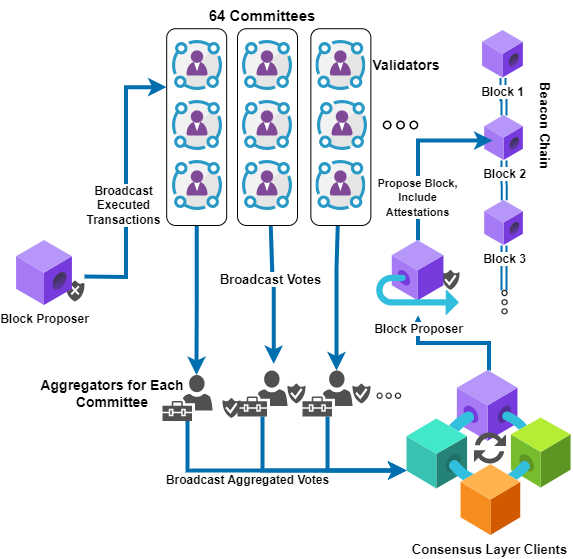
\includegraphics[width=13cm,center]{Figures/AttestationsDiragram.png}
    \caption{A flow diagram visualising the new block proposal and attestation process in PoS Ethereum}
    \label{Figure:AttestationsDiragram}
\end{figure}

 % ---CAN BE REMOVED**
\textit{Staking ETH}

In Ethereum, an \textbf{epoch} comprises 32 slots ($\sim$6 minutes). The algorithm judges each validator's actions and dishes out rewards and penalties at the end of each epoch accordingly. Validators staking ETH and running Validators earn transaction fees and tips but also risk losing part of their stake through \textbf{slashing} or incurring \textbf{offline penalties}.

% CAN BE CUT**
% The Merge switched Ethereum's security model's reliance on  computational power to \textbf{economic power}. Malicious attackers now need 51\% of the economic power of the entire network instead of computational power to conduct a successful attack. The severe economic punishments mentioned earlier help to keep the network more secure than ever before while massively reducing its energy consumption. 


% ----------------------------------------------------------------------

% The version of the ledger stored by Full Nodes and validators is periodically pruned so that they don't hold the entire chain dating back to the Genesis block. \textbf{Archive Nodes} are a type of node that maintain an exact and complete copy of the entire blockchain dating back to the Genesis block. 

% Apart from users looking to earn ETH or altruistic users wanting to secure the Ethereum network, not many users have the incentive to invest the time and resources to run a Full Node. This is why most users end up using centralised 3rd party hosted nodes. Client wallets like MetaMask and MyEtherWallet connect to a remote node in a non-cryptographically proven matter. New lighter node types, such as Light Nodes, were introduced to help make Ethereum accessible to more users, which in turn also makes the network more secure.

% \textbf{Light Nodes :}
% These are nodes that don't stake Ethereum. Instead, they are just used for accessing the network along with storing and processing the validation of the blocks within the network. These rely on full nodes as intermediaries to receive up-to-date information about the state of the blockchain. In essence, they are spectator nodes that constantly monitor the network and are witnesses that all activity complies with the rules.

% Because they are up-to-date nodes, they are allowed to interact with the Ethereum blockchain.  All they require is a simple installation of an ETH 2.0 node and a connection to the internet. This means the minimum requirements for the hardware required to run a light node is minimal and can be run on mobile devices.

% By design, they don't need to store or process the same amount of information that full nodes do. PoW light nodes only used download the headers of each block and were able to trace back. PoS light nodes also has to keep track of validators and their balances to stay on the chain with the most stake. This small amount of information allows light nodes to operate in a trust-minimised manner.

% % CAN BE CUT**
% \subsection{Client Types}

% Client software is software that facilitates inter-node communication in a peer-to-peer manner.

% \textit{Execution Layer Clients}

% EL clients,  formerly known as 'Eth 1' clients, come in the form of open-source community-maintained software. A diverse share of client software being run on nodes across the network is favourable as it reduces single points of failure.

% Some popular EL clients include Geth, Nethermind, Besu and Erigon \cite{EthereumEthereum.org}. 

% \textit{Consensus Layer Clients }

% Following 'The Merge', CL clients, known as 'Eth 2' clients, facilitate the new PoS consensus-forming mechanism, securing the Ethereum blockchain.

% Some popular CL clients include Prysm, Lighthouse, Teku, Nimbus and Lodestar \cite{EthereumEthereum.org}. 
% % __
\subsection{Synchronisation} 
\label{SyncLitRev}

Synchronisation refers to a new node catching up to the latest version of the Ethereum blockchain ledger by retrieving the most up-to-date information during bootstrapping. Data received from peer nodes is cryptographically verified and used to build a local copy of the ledger.

PoS Ethereum relies on the Consensus Layer for handling consensus logic and block propagation. Thus, synchronisation is a shared process between the EL and CL client. In order for the EL client to start verifying and syncing a local copy of the blockchain, the CL client has to download the appropriate block headers. Once the chain of block headers is formed and validated, the remaining block information is downloaded, which is typically the most time-consuming step \cite{2022DeveloperGo-ethereum}.

There are different types of syncing modes, including Full, Snap, Fast and Light Sync.

\textit{Full Sync }independently verifies the block provenance by re-executing the transactions starting at the Genesis Block. However, in a Full Node, only the latest 128 blocks are actually stored, along with a few checkpoints representing older blocks \cite{EthereumEthereum.org}. 

\textit{Snap Sync} works similarly to a Full Sync, except it starts at a much more recent checkpoint to start its verification up to the front of the chain \cite{2022DeveloperGo-ethereum}.

Synchronisation time varies depending on the client software chosen, as well as the node's hardware configuration. Syncing times can range from 12 hours up to 6 days or more (see Appendix B).
% -_____________________________________________________________________________

% __________________________________________________________________________________________-
% -_____________________________________________________________________________

% __________________________________________________________________________________________-

\section{Carbon Emissions of Blockchain Technology }

Bitcoin, the world's largest cryptocurrency, currently holds a market cap of \$588 billion, with Ethereum trailing behind narrowly (\$242 billion market cap) \cite{BitcoinCoinMarketCap}. Most cryptocurrencies still rely on the Proof-of-Work mechanism, which by design uses energy-intensive processes to secure the network. Hence, it should not be surprising that they have huge adversarial effects on the environment. Empirical findings using the ARDL model (used to analyse the long-term relationship between variables) show that increasing the volume of trading all cryptocurrencies results in higher energy consumption, with long-term effects on the environment \cite{Schinckus2020Crypto-currenciesConsumption}. 

While the benefits of using decentralised transactional systems appeal to many, it has become synonymous with inefficiency and disproportionate energy consumption \cite{DeVriesBitcoinsProblem}. Digiconomist's index suggests that if Bitcoin's energy was to be compared to that of entire countries, it would rank 38$\mathrm{^{th}}$ in the world, finishing ahead of large countries like Chile and Bangladesh \cite{BitcoinDigiconomist}. The high energy costs associated with the inherent have become hugely problematic, inhibiting the wider adoption of cryptocurrencies. 

To put this in perspective, comparisons between cryptocurrencies and traditional centralised transactional systems, such as Visa, are often drawn \cite{Kohli2023AnSolutions}. However, due to their centralised nature, these systems will always be more efficient, as shown in \fref{Figure:CarbonEmissionsPlot}.

\begin{figure}[!htb]
    \centering
    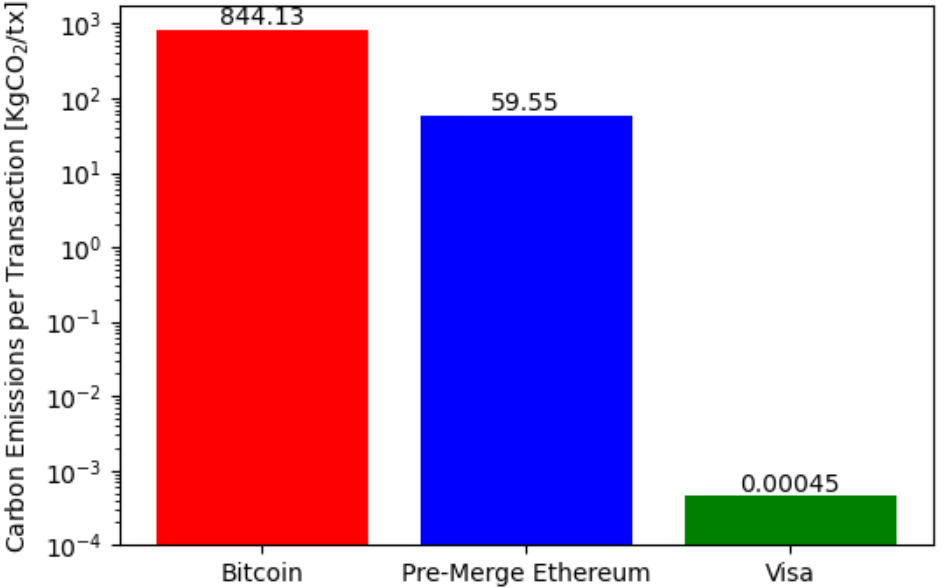
\includegraphics[width=13cm,center]{Figures/CarbonEmissionsPlot.png}
    \caption{Carbon emissions per transaction for Bitcoin, Ethereum 1.0 and Visa plotted on a logarithmic scale. Code is in Appendix C. Source: \cite{Kohli2023AnSolutions} }
    \label{Figure:CarbonEmissionsPlot}
\end{figure}

These carbon emissions can be used as a proxy for environmental damage \cite{2022VisaReport}, which is associated with high energy consumption and makes PoW cryptocurrencies unsustainable.

Besides cryptocurrencies, blockchain technology is experiencing significant growth in the drug-supply chain industry \cite{Labaran2021TheNigeria}. This sector features the adoption of large-scale blockchain solutions that boast low-energy usage, found in \tref{Table:DrugSupplyImplementations}. Consequently, the answer to reducing high energy consumption may be found in these innovative applications of blockchain technology, most of which employ non-PoW mechanisms.

\begin{table}[!htb]
\centering
\begin{tabular}{|l"l|l|l|l|l|}
\hline
\textbf{Topic} &
  \textbf{\begin{tabular}[c]{@{}l@{}}Vaccine \\ Delivery \\ Solution\end{tabular}} &
  \textbf{\begin{tabular}[c]{@{}l@{}}Medication \\ Anti-fraud \&\\ Traceability\end{tabular}} &
  \textbf{\begin{tabular}[c]{@{}l@{}}‘Everyware’\\ Platform\end{tabular}} &
  \textbf{\begin{tabular}[c]{@{}l@{}}Analysis of \\ Blockchain in \\ Healthcare\end{tabular}} &
  \textbf{\begin{tabular}[c]{@{}l@{}}Drug \\ Traceability\\ Solution\end{tabular}} \\ \thickhline
\textbf{\begin{tabular}[c]{@{}l@{}}Blockchain \\ Platform\end{tabular}} &
  Ethereum 1.0 &
  Ethereum 1.0&
  Hedera &
  \begin{tabular}[c]{@{}l@{}}Hyperledger\\ Fabric\end{tabular} &
  Ethereum 1.0 \\ \hline
\textbf{\begin{tabular}[c]{@{}l@{}}Consensus \\ Algorithm\end{tabular}} &
  PoW &
  \begin{tabular}[c]{@{}l@{}}practical\\ Byzantine\\ fault tolerance\end{tabular} &
  \begin{tabular}[c]{@{}l@{}}Hashgraph\\ Consensus\end{tabular} &
  \begin{tabular}[c]{@{}l@{}}Redundant\\ Byzantine \\ fault tolerance\end{tabular} &
  PoW \\ \hline
\textbf{\begin{tabular}[c]{@{}l@{}}Type of \\ Operations\end{tabular}} &
  \begin{tabular}[c]{@{}l@{}}Public   \\ Permissioned\end{tabular} &
  \begin{tabular}[c]{@{}l@{}}Public   \\ Permissioned\end{tabular} &
  \begin{tabular}[c]{@{}l@{}}Public \\ Permissioned\end{tabular} &
  \begin{tabular}[c]{@{}l@{}}Private   \\ Permissioned\end{tabular} &
  \begin{tabular}[c]{@{}l@{}}Public\\ Permissioned\end{tabular} \\ \hline
\textbf{Currency} &
  Ether &
  None &
  None &
  None &
  Ether \\ \hline
\textbf{\begin{tabular}[c]{@{}l@{}}Off-chain \\ storage\end{tabular}} &
  Yes &
  None &
  Yes &
  None &
  Yes \\ \hline
\textbf{\begin{tabular}[c]{@{}l@{}}Customisable \\ Component\end{tabular}} &
  \begin{tabular}[c]{@{}l@{}}Ethereum\\ Smart \\ Contracts\end{tabular} &
  \begin{tabular}[c]{@{}l@{}}Ethereum\\ Smart\\ Contracts\end{tabular} &
  Yes &
  \begin{tabular}[c]{@{}l@{}}Docker\\ Container\end{tabular} &
  \begin{tabular}[c]{@{}l@{}}Ethereum\\ Smart \\ Contracts\end{tabular} \\ \hline
\textbf{\begin{tabular}[c]{@{}l@{}}Energy \\ Consumption\end{tabular}} &
  High &
  Low &
  Very Low &
  Low &
  High \\ \hline
\textbf{Source} &
  \cite{Musamih2021Blockchain-BasedVaccines} &
  \cite{Zhu2020ATraceability} &
  \cite{Platform}, \cite{TechnologyLtd} &
  \cite{Mettler2016BlockchainHere} &
  \cite{Musamih2021AChain} \\ \hline
\end{tabular}
\caption{Several implementations of drug-supply chain solutions that use blockchain technology, with 3 implementations using high-energy Ethereum 1.0.}
\label{Table:DrugSupplyImplementations}
\end{table}

However, newly established independent blockchains, for cryptocurrencies or provenance purposes, often struggle with achieving decentralisation benefits, facing security breaches or centralisation issues. 51\% attacks occur when a malicious miner or group controls over 50\% of a network's computational power. Small blockchains with few participants are more vulnerable as it is easier for a malicious actor to acquire the necessary computational power, leaving the blockchain susceptible to tampering and theft \cite{Redman2021PrivacyErased}.





% _______________________________________________________________
% -_____________________________________________________________________________

% __________________________________________________________________________________________-
% -_____________________________________________________________________________

\subsection{Mathematical Modelling}
\label{MathematicalModellingLitRev}

Mathematical modelling simplifies complex systems and tests hypotheses by making some assumptions. There are various approaches for scientific model building, including descriptive and rule-based modelling \cite{SayamaINTRODUCTIONSYSTEMS}. This study employs the latter.

\textbf{Rule-Based Modelling} focuses on formulating dynamic rules and limitations that can explain the behaviour of a system over time. This is usually done using quantitative methods.

Turning observations into mathematical equations can be challenging, especially when dealing with unique properties like large networks and nonlinearity. When modelling complex systems, according to \cite{SayamaINTRODUCTIONSYSTEMS}, it's crucial to remember the following four factors:

\begin{itemize}
    \item The key research questions that need to be addressed
    \item To answer the research questions, what scale is most appropriate to describe the systems, microscopic or macroscopic
    \item How the system is structured
    \item What are all the possible states of the system, and how it changes over time
\end{itemize}

This study will use the microscopic details of the Ethereum protocol (how attestations are handled) to model its macroscopic effects at scale (increase in overall energy usage) \cite{MarionAnModelling}. 



% ____________________________________________________________________---

% ______________________________________________________________________________
% -_____________________________________________________________________________

% __________________________________________________________________________________________-


\section{Modelling PoW Energy Consumption}

This subsection analyses various papers on the energy consumption of blockchain, loosely following the structured literature review steps outlined by \cite{Crosby2015BlockChainBitcoin}.

Most papers in this niche field emphasise Bitcoin and PoW cryptocurrencies. There is a clear gap in the literature for more work to be done on modelling the electricity consumption of non-PoW blockchains, as this study intends to do.
% -_____________________________________________________________________________

Paper \cite{Sedlmeir2020TheMyth} attributes almost all the energy consumed by PoW blockchains to the PoW consensus mechanism alone. Other factors contribute a negligible amount of energy in comparison. However, estimating the energy consumption of blockchain consensus mechanisms can be challenging due to the scarcity of accurate information on the number of network participants and their hardware configurations. The same study also confirms that PoW blockchains consume a disproportionate amount of energy relative to the actual utility they offer. When comparing PoW electricity estimates to those of non-PoW blockchains, the results were several orders of magnitude lower for non-PoW blockchains \cite{Sedlmeir2020TheMyth}. 

\begin{figure}[h]
    \centering
    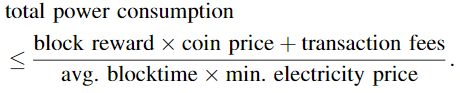
\includegraphics[width=8cm,center]{Figures/SimplePoWModel.png}
    \caption{A simple model estimating the upper bound of electricity consumption of a PoW blockchain. Source: \cite{Sedlmeir2020TheMyth} }
    \label{Figure:SimplePoWModel}
\end{figure}

Energy consumption in many PoW-focused papers is attributed to metrics like block rewards, coin price, transaction fee, average block time and hashing difficulty which are all publicly available and reliable metrics, \cite{Mcdonald2022EthereumEstimate}. Such a model is shown in \fref{Figure:SimplePoWModel}. On the contrary, non-PoW consensus algorithms have such a much small energy footprint that cannot solely be attributed to its consensus mechanism but also to various factors associated with maintaining a large decentralised network, as explained in \sref{LitRevExistingModels}. 

% -_____________________________________________________________________________
Another study combined publicly available data with a small number of direct measurements from a small testbed network to derive a joule per hash value based on \cite{Cole2018ModelingAlgorithms}. Using a LASSO (Least Absolute Shrinkage and Selection Operator) regression model, the researchers were able to estimate the energy usage of PoW cryptocurrencies with 92\% accuracy. The same cannot be done for PoS blockchains due to the lack of data availability and the vast range of factors affecting its energy consumption outside of the consensus protocol itself.

Digiconomist \cite{BitcoinDigiconomist} and CBECI \cite{CambridgeCBECI} are two well-known real-time models used to estimate the energy consumption of Bitcoin. These are highly credible models and have been referenced many times in the wider literature, such as \cite{Cole2018ModelingAlgorithms}, \cite{Lei2021BestRecommendations}, and \cite{Erdogan2022AnalyzingSustainability}, \cite{Platt2022TheProof-of-Work}, respectively. Both models use live tracking of Bitcoin's price and mining hash rate to maintain accuracy but take different approaches to arrive at similar estimates. Digiconomist's top-down approach estimates the total revenue earned by USA-based Bitcoin miners. It assumes that 60\% of this revenue is spent on operational costs, primarily electricity, in the case of PoW. By using the global average electricity costs, the model is able to calculate Bitcoin's energy consumption. In contrast, CBECI uses a bottom-up approach, focusing on selecting contemporary mining equipment that maximises the number of hashes computed per Joule of energy used. The model then uses a profitability threshold to extrapolate Bitcoin's annual electricity consumption. This study will take a bottom-up approach to develop a model for non-PoW Ethereum.


% __________________________________________________________________________________________-
% __________________________________________________________________________________________-


\subsection{ Electricity Consumption of PoS Blockchains }
\label{LitRevExistingModels}

There is an even larger gap in the literature on this emerging research topic. This subsection analyses the work done in this area and why it needs improvement.

A study by Powell et al. \cite{Powell2021AWARENESSBLOCKCHAIN}, aimed at making recommendations for building greener blockchains, suggested a simple formula to calculate the energy of the Polkadot blockchain that employs PoS consensus. The model was the first of its kind, and it follows: 
\begin{align}
   \boldsymbol{\mathrm{\text{Polkadot Energy Consumption } = }}
   &\boldsymbol{\mathrm{\text{ Energy per server }* \text{ number of servers } } } \nonumber\\
   &\boldsymbol{\mathrm{* \text{ 24 hours } *\text{ 365 days }}} \nonumber
\end{align}

\textit{The UCL Model } 

A recent study by the UCL Centre for Blockchain Technologies \cite{PlattDiscussionProof-of-Work} improved upon this equation by establishing a mathematical relationship between the number of validators, network load and hardware configurations to estimate the energy consumption of the PoS consensus protocol, in isolation. Their approach was to build upon past literature using new data sets from various sources, including empirical data from CCRI report \cite{CryptoCarbonRatingsInstitute2022TheNetwork} and other publicly available metrics, while avoiding time-consuming first-hand experimentation, just like this study aims to do. 

\begin{align}
   \boldsymbol{\mathrm{\text{Energy Per Transaction} = }}
   &\boldsymbol{\mathrm{\frac{\text{ Energy per Validator }* \text{ Number of Validators } }{\text{ Number of Transactions }}} } \nonumber\\ \nonumber
\end{align}

Their generalised model performs well for a few different PoS blockchains, with Ethereum 2.0 being one of them. In fact, R3, a private company that runs the Corda blockchain have also used the UCL  equation to estimate Corda's energy consumption \cite{JustBlog}. However, amidst this generalisation, the UCL study makes a critical error by not differentiating between operating validators clients (currently $\sim$500,000 \cite{EthereumEthereum.orgc}) and Full Nodes ($\sim$15,000 \cite{NodewatchAnalytics}). Their model only considers Full Nodes, which is an error repeated in an updated paper by the same researchers \cite{IbanezTheExpansion}, likely due to the aim of generalisation and modelling only the PoS consensus mechanism's energy consumption in isolation. Thus, incomplete in its calculation of network-wide energy consumption by ignoring factors such as the validators that are actively participating in consensus-forming processes. 

The original UCL study also relies on speculative assumptions as it was written before Ethereum’s upgrade to PoS consensus (now the world’s largest PoS blockchain). Hence, the most significant PoS blockchain was not included in its study.

The future work mentioned by the researchers closely matches the focus of this study, which aims to build a more comprehensive model by incorporating additional factors like active validators.


\textit{The CCRI Model } 
\label{CCRIModelLitRev}

The state-of-the-art research conducted by Crypto Carbon Ratings Institute focuses specifically on the energy consumption of post-merge PoS Ethereum. It provided the most up-to-date empirical data that has been cited in other studies such as this one \cite{CryptoCarbonRatingsInstitute2022TheNetwork}. Its researchers decided on 6 commodity hardware configurations that were run idly for base power consumption figures. Then each major EL and CL client software was run separately, taking 48-hour electricity measurements. The data helped develop their equation (detailed in \sref{CCRIBaseEqnSection}), which was formulated using a combination of experimental and prior domain knowledge. The model's accuracy was confirmed by comparing the actual measurements from Full Nodes to the model's estimations, which were found to be highly precise.

Assumptions and shortcomings of this study:
\begin{enumerate}
    \item While various measurements were combined to represent running a Full Node, the next step of running a validator client was not taken. This is because the energy expenditure of operating a validator client on top of a Full Node was assumed to be negligible and also due to the requirement of staking 32 ETH.
    
    \item The synchronisation energy consumed whilst bootstrapping Full Nodes was not considered.
    
    \item Other node types, such as Light and Archive Nodes, were not considered, presumably due to assuming that they would have negligible effects.

    \item The electricity measurements were collected using computer software rather than hardware meters, and no information was provided on the type of power supply and mainboard used in the experiment. Therefore, the software measurements only account for the electricity used by the computer itself and do not factor in the power drawn 'At-Wall' or any other electrical inefficiencies \cite{Warkozek2012ACenters}.
\end{enumerate}
 


% -_____________________________________________________________________________


% Quick intro on AVX operations, what is TDP and why that is the upper limit of CPU power consumption
% AVX instructions enable the processor to perform multiple floating-point operations at the same time, resulting in faster computation and improved performance. \cite{Schuchart2016TheScale}

% ______________________________________________________________________________
% -_____________________________________________________________________________

% __________________________________________________________________________________________-

% \section{Key Points Covered}
